For the implementation, initially the possibilities for Cloud Servers were taken in account, like Amazon, Linode and Heroku. Among those, the one shown best fit for the practical implementation of an operational prototype of our mechanism was Heroku. \cite{heroku} is a Cloud solution which offers the infrastructure to the hosting service we need. It also allows the use of frameworks like Django, Ruby on Rails (RoR) and node.js. Between the alternatives, we chose the RoR solution, due to the fact that we have greater experience in this technology, but our mechanism is not framework or language dependent, an as such, our experiment could be reproduced in any other alternative of language and framework.

The architecture of the RoR Framework in completely based on the Model View Controller (MVC) paradigm, making it easier to organize the modules in our mechanism. This way, the code structure is composed by parts of Model, View and Control. The \textbf{Model} part concerns everything related to the data -- how it is stored, fetched and related. The \textbf{View} part is related to any graphics the application may show. Least, \textbf{Controllers} handle data, they concern the logical and functional part of the code. They also make the bridge between Model and View, allowing the data to transit in both ways.

Thus, the Traffic Analyzer (TA) submodule of the mechanism belongs to the Controller part. A request to the application will be intercepted by this component, which will probe some statistic data, and soon after, will call the controller responsible by the functioning of the application itself. It is important to notice, however, that time spent in this controller is undermost, only the necessary to process a few equations and store the results for statistical control. Just in case this process may affect the functioning of the application, it might be performed in background.

Case the TA detects the existence of a possible attack, a new instance of the application in the Cloud is created by the NAI submodule, paralyzing the original application, that becomes just a traffic redirector. The re-instantiantion process for an application may happen in two ways. The most simple approach would be that the second application already exists, but with no allocated resources. However, this approach does not behave in the best way possible for a recursive scenario of re-instantiation. The second approach concerns hosting the project in a GitHub repository, so it may be cloned into the second instance via ruby code.

One interesting particularity of the RoR framework is the existence of a routes configuration file. The implementation of the TR submodule will be made using this file, called \textit{routes.rb}. In order to show any dynamic page from the application, this file is inevitably requested. Thus, that is the ideal place to add clients to a blacklist and filter clients blocked by the BM. When redirecting traffic to a new instance, a new entry should be added, blocking the client who sent the request for a certain time.

The blacklist itself and many others control variables will be managed by the database in the \emph{Cloud}~\cite{redis}. Such database if famous by its simplicity and efficiency. It basically maps \textbf{key} and \textbf{value}, offering reading and writing time equivalent to a hash. This way, one option to implement the blacklist in Redis is using the client's IP as a key, and the time it will be blocked is the value mapped by it. The time to check a client is O(1), for it is, abstractly, a hash, and this is excellent for a mechanism that will filter all the incoming traffic. A structured view of the functions performed by the proposed architecture is described in the flux diagram illustrated in the figure~\ref{fig:dfd}.

\begin{figure}[t!]
	\centering
	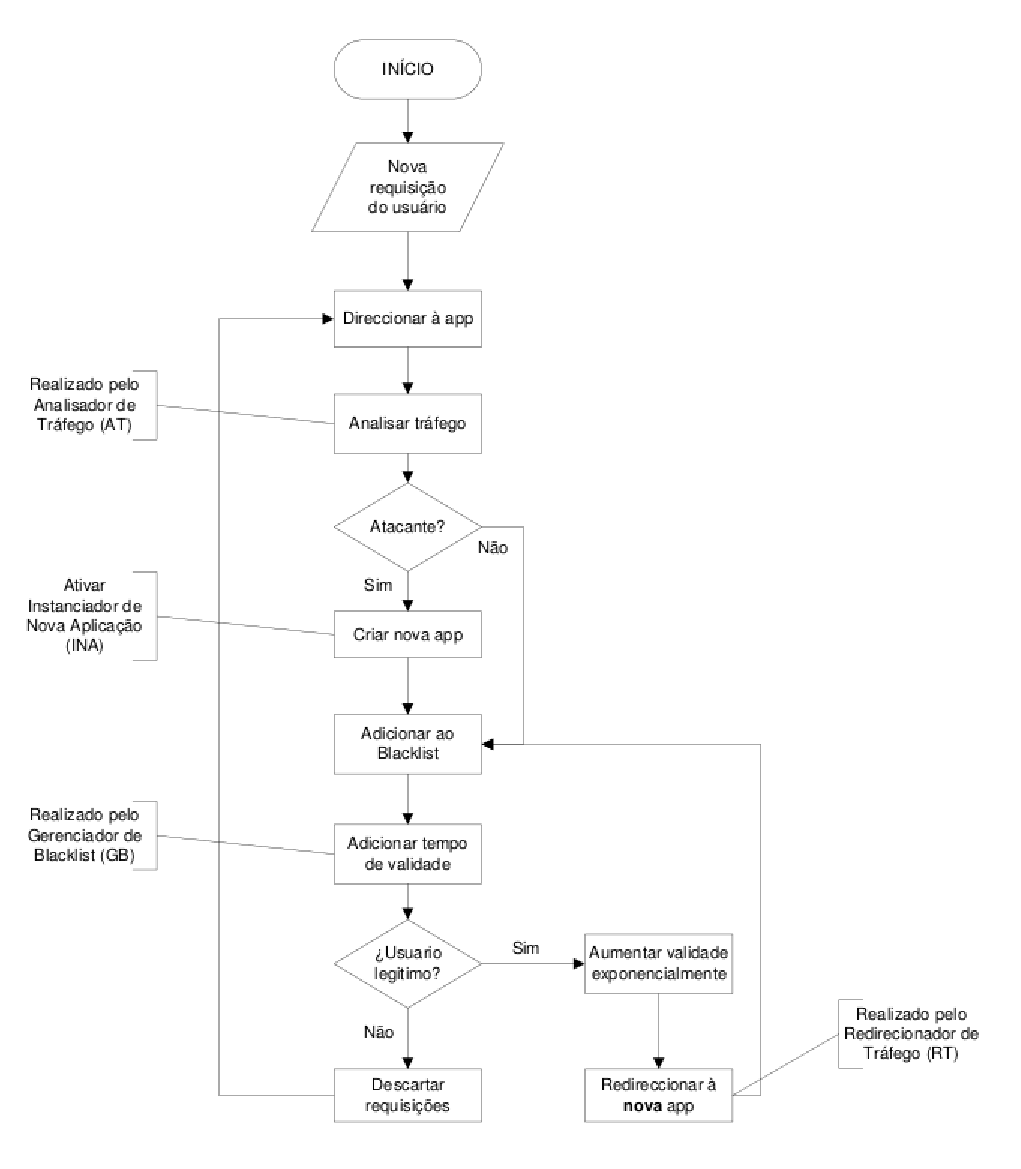
\includegraphics[width=0.90\textwidth]{images/dfd.eps}
	\hskip 1cm
	\caption{Functions of the DDoS mitigating architecture}
	\label{fig:dfd}
\end{figure}

Least, an interesting feature of using Heroku are the many add-ons it offers. I particular, there is one add-on called New Relic which is responsible for collecting data for performance analysis. This add-on will make it possible to know precisely what is going on in every instance of the application in a Cloud from a internal perspective. Thus, we will be able to probe data of not only the external perspective (which is the user perspective), but also the internal view.